\documentclass[]{llncs}

\usepackage{tikz}
\usepackage{pgfplots}
\usepackage{subfig}
\usepackage{enumitem}
\usepackage{verbatim}
\usepackage{biblatex}
\usepackage{filecontents}
\usepackage[absolute]{textpos}
\usepackage{dsfont}

\usetikzlibrary{positioning}

\begin{filecontents}{bib.bib}
@inproceedings{conf/alenex/ChimaniZ14,
  added-at = {2014-02-12T00:00:00.000+0100},
  author = {Chimani, Markus and Zeranski, Robert},
  biburl = {https://www.bibsonomy.org/bibtex/26e5cfdc3e8cb806f9be58c1f08ab3867/dblp},
  booktitle = {ALENEX},
  crossref = {conf/alenex/2014},
  editor = {McGeoch, Catherine C. and Meyer, Ulrich},
  ee = {http://dx.doi.org/10.1137/1.9781611973198.8},
  interhash = {a5b9d9206da585e35cc9d30e3f047513},
  intrahash = {6e5cfdc3e8cb806f9be58c1f08ab3867},
  isbn = {978-1-61197-319-8},
  keywords = {dblp},
  pages = {73-85},
  publisher = {SIAM},
  timestamp = {2015-06-19T02:24:42.000+0200},
  title = {An Exact Approach to Upward Crossing Minimization.},
  url = {http://dblp.uni-trier.de/db/conf/alenex/alenex2014.html#ChimaniZ14},
  year = 2014
}

@electronic{bollobas98,
  abstract = {The time has now come when graph theory should be part of the education of every serious student of mathematics and computer science, both for its own sake and to enhance the appreciation of mathematics as a whole. This book is an in-depth account of graph theory, written with such a student in mind; it reflects the current state of the subject and emphasizes connections with other branches of pure mathematics. The volume grew out of the author's earlier book, Graph Theory -- An Introductory Course, but its length is well over twice that of its predecessor, allowing it to reveal many exciting new developments in the subject. Recognizing that graph theory is one of several courses competing for the attention of a student, the book contains extensive descriptive passages designed to convey the flavor of the subject and to arouse interest. In addition to a modern treatment of the classical areas of graph theory such as coloring, matching, extremal theory, and algebraic graph theory, the book presents a detailed account of newer topics, including Szemer'edi's Regularity Lemma and its use, Shelah's extension of the Hales-Jewett Theorem, the precise nature of the phase transition in a random graph process, the connection between electrical networks and random walks on graphs, and the Tutte polynomial and its cousins in knot theory. In no other branch of mathematics is it as vital to tackle and solve challenging exercises in order to master the subject. To this end, the book contains an unusually large number of well thought-out exercises: over 600 in total. Although some are straightforward, most of them are substantial, and others will stretch even the most able reader.},
  added-at = {2015-05-19T09:19:57.000+0200},
  address = {New York},
  author = {Bollob\'{a}s, B\'{e}lla},
  biburl = {https://www.bibsonomy.org/bibtex/27b84cb41ef679da77300486d9f6f0916/ytyoun},
  doi = {10.1007/978-1-4612-0619-4},
  interhash = {875127e4e9980d87bf0bdeab7fa97559},
  intrahash = {7b84cb41ef679da77300486d9f6f0916},
  isbn = {9781461206194},
  keywords = {bollobas characteristic eigenvalues graph.theory hoffman monotonicity polynomial rayleigh textbook},
  publisher = {Springer},
  refid = {682118471},
  timestamp = {2017-11-10T06:33:22.000+0100},
  title = {Modern Graph Theory},
  year = 1998
}

@article{journals/corr/abs-1808-10519,
  added-at = {2018-09-04T00:00:00.000+0200},
  author = {Bekos, Michael A. and Förster, Henry and Geckeler, Christian and Holländer, Lukas and Kaufmann, Michael and Spallek, Amadäus M. and Splett, Jan},
  biburl = {https://www.bibsonomy.org/bibtex/2e13a59afe7afa2da70a3d34ebc7993c1/dblp},
  ee = {http://arxiv.org/abs/1808.10519},
  interhash = {0703b4c6a706aafb35707a22e420381f},
  intrahash = {e13a59afe7afa2da70a3d34ebc7993c1},
  journal = {CoRR},
  keywords = {dblp},
  timestamp = {2018-09-05T11:36:29.000+0200},
  title = {A Heuristic Approach towards Drawings of Graphs with High Crossing Resolution.},
  url = {http://dblp.uni-trier.de/db/journals/corr/corr1808.html#abs-1808-10519},
  year = 2018
}

@inproceedings{conf/gd/DemelDMRW18,
  added-at = {2019-12-17T16:50:25.000+0100},
  author = {Demel, Almut and Dürrschnabel, Dominik and Mchedlidze, Tamara and Radermacher, Marcel and Wulf, Lasse},
  biburl = {https://www.bibsonomy.org/bibtex/24d53ae536166435e13c78aeb2025d574/duerrschnabel},
  booktitle = {Graph Drawing},
  crossref = {conf/gd/2018},
  editor = {Biedl, Therese C. and Kerren, Andreas},
  ee = {https://doi.org/10.1007/978-3-030-04414-5_20},
  interhash = {44c9d5616b9daf6501104053f403cfdc},
  intrahash = {4d53ae536166435e13c78aeb2025d574},
  isbn = {978-3-030-04414-5},
  keywords = {crossing_angle_maximization greedy_heuristik myown},
  pages = {286-299},
  publisher = {Springer},
  series = {Lecture Notes in Computer Science},
  timestamp = {2019-12-17T16:50:25.000+0100},
  title = {A Greedy Heuristic for Crossing-Angle Maximization.},
  url = {http://dblp.uni-trier.de/db/conf/gd/gd2018.html#DemelDMRW18},
  volume = 11282,
  year = 2018
}

@incollection{reference/algo/Nikolov16a,
  added-at = {2016-04-28T00:00:00.000+0200},
  author = {Nikolov, Nikola S.},
  biburl = {https://www.bibsonomy.org/bibtex/213bf0a108b9daa193eb6bed0a9fa9198/dblp},
  booktitle = {Encyclopedia of Algorithms},
  ee = {http://dx.doi.org/10.1007/978-1-4939-2864-4_649},
  interhash = {63071df6dfaf484158873ecb3f507c72},
  intrahash = {13bf0a108b9daa193eb6bed0a9fa9198},
  keywords = {dblp},
  pages = {2162-2166},
  timestamp = {2016-04-29T11:41:13.000+0200},
  title = {Sugiyama Algorithm.},
  url = {http://dblp.uni-trier.de/db/reference/algo/algo2016.html#Nikolov16a},
  year = 2016
}

@misc{np,
  author = {Garey, M.R.;Johnson, D. S.},
  title = {Crossing number is NP-complete},
  ee = {http://dx.doi.org/10.1137/0604033},
  pages = {312-316},
  year = 1983
}

\end{filecontents}

\addbibresource{bib.bib}

\begin{document}
    \title{Graph Drawing Contest 2020 \\
           Crossing Minimization with Randomness}
    \author{Sebastian Benner}
    \institute{Universität Kassel FB 16}
    \maketitle
    
    \abstract{Drawing graphs with the minimal amount of edge-crossings is a NP complete problem. Additional constraints placed upon the drawing, namely being a straight-line upwards drawing, do not reduce this complexity. To approximate a solution for this problem within a certain time frame and with the least amount of edge-crossings possible, a multi-step algorithm based mostly on random displacements is proposed. While some limitations are necessary, the best results were achieved by only preventing erroneous positions and only the most bare bone limitations. In addition the work contains some pointers for further improvements and adaptation to different constraints placed upon the drawing.}

    \section{Introduction} 	
	Calculating the minimal number of crossings present in all possible drawings of a graph is a hard problem. In~\cite{np} it was shown to be NP-complete. Likewise, it is equally as hard to find such a drawing.
	
	To circumvent this problem, algorithms are designed to find drawings with close to if not equal to the minimal amount of crossings. The annual Graph Drawing Contest\footnote{http://mozart.diei.unipg.it/gdcontest/contest2020/challenge.html} is an open challenge to design such an algorithm for optimized graph drawings. The exact criteria for such a drawing are changed every couple of years, but both the current and last contest aimed for minimal crossings. The Live Challenge will contain between five to ten acyclic directed graphs with up to a few thousands nodes each. All resulting layouts must be submitted within one hour of the graphs being handed out.

Besides the main criterion additional constraints are placed on the drawings:
\begin{itemize}
	\item Each edge must be a straight upward facing line, meaning the source of each directed edge must be lower than the target.
	\item Each node must be placed upon a grid of given size.
	\item Crossings between a node and an edge are not permitted, as well as overlapping nodes.
\end{itemize}
The constraints do not change the complexity of the problem. In~\cite{conf/alenex/ChimaniZ14} it was shown that determining whether or not a directed acyclic graph even allowed a upwards drawing without any crossings is already NP-complete - a problem that can be solved more easily for undirected graphs.

After all resulting graphs are collected, for each of the original graphs a best drawing is determined with all the other graphs receiving a weighted score based on the difference in edge-crossings. The highest overall score wins the contest. Each team has to bring its own hardware to run their respective algorithm, meaning there is no limitation in terms of tools used and the given time to solve the task can be counterbalanced by more powerful hardware.

For at least three consecutive years the winning algorithm was based on randomness. The aim of this work is to iterate on these winning entries and to provide a lightweight algorithm much more focused on the random aspect than before.

The rest is structured as follows: Section 2 and 3 will go through the notation needed and related work respectively. Afterwards, section 4 will propose the algorithm with an evaluation in the next chapter. What follows is a section containing both failed approaches as well as pointers for follow-up work not bound to the constraints of the contest. Finally, section 6 will give a conclusion.

	\section{Mathematical Foundation}
	A $graph\;G$ is defined as an ordered pair $(V, E)$ of $vertices\;V$ and $edges\;E$. Edges are unordered pairs of two vertices $\{x,y\}$, said to $join$  them, and therefore $E$ is a subset of $V \choose 2$. In the special case where edges are ordered pairs $(x,y)$ with $x$ as $source$ and $y$ as $target$ the graph $D$ is called $directed$ graph or $digraph$. We call the number of vertices the $order$ of $G$ and the number of edges the $size$ of $G$. $V(G)$ and $E(G)$ are the sets of vertices and edges of $G$ respectively, $x \in V(G)$ with vertex $x$ can be written as $x \in G$ while $\{x, y\} \in E(G)$ with undirected edge $\{x,y\}$ is written as $\{x,y\} \in G$. For a more comprehensive explanation I refer to the book $Modern$ $Graph$ $Theory$~\cite{bollobas98} upon which this notation is based on.

A $drawing$ is a visual representation of a graph through a $layout$, which itself is a mapping $V \longrightarrow X_1 \times X_2$ with $X_1,X_2 \subset \mathds{N}$ as two-dimensional coordinates $(x_1, x_2)$. Directed edges are drawn as straight arrows between their respective nodes pointing from the source to the target. A drawing is called $upwards$ if $x_{2_{target}} > x_{2_{source}} \forall (target, source) \in E$. A $node$-$overlap$ is defined by two nodes having the same coordinates. $Edge$-$crossings$ and $node$-$crossings$ occur when a edge is drawn through another edge or a node respectively.

	\section{Related Work}
    There have been many works on minimizing the crossings in a drawing. This section will go through the most significant contributions to the algorithm presented here, many of them bear a connection to the contest, which this work is aimed at.

	While not aiming at the same goal, the algorithm in~\cite{journals/corr/abs-1808-10519} served as a basis for the last years winner. The aim was to create a drawing with the largest minimum angle, called the resolution of $G$,  possible. To achieve this the algorithm build and maintained two sets: all nodes and only such nodes that are deemed critical for the current resolution of $G$. Critical are all nodes connected with edges involved in minimal angles. In each iteration either a node from the set of all critical nodes is chosen uniformly or inverse proportionally to its proximity to a critical nodes from the set of all nodes. To determine the new position of a node rays are used which are cast out uniformly distributed in all directions with the best result becoming the new position. Combined with a energy-based base drawing and some tweaks to avoid local minima, the algorithm proved itself and also won its respective year.

	Another winning contribution to a different year with the same aim as before is found in~\cite{conf/gd/DemelDMRW18}. An algorithm to create a drawing with the largest possible minimum angle. Starting from a force directed base drawing the algorithm is greedily selecting the minimal crossing from the current drawing. A random vertex is chosen and displaced to the optimal position within a square around the original position to achieve the maximal local crossing angle. The size of the square is decreased with each iteration.

    \section {Proposed Algorithm}
	The following algorithm is a multi-step procedure. The first step is to apply a base drawing, which is chosen to achieve the best results in the least amount of time. While it is not needed, starting from a local minima reduces the iterations for the second step. Said step consists of random displacements to produce improvements or no changes at all for a single randomly chosen node each iteration. The second step was designed to run as efficient as possible for the maximum amount of displacements within the time frame.

    \subsection{Base Drawing}
	The base drawing used in this algorithm is the $Sugiyama\;Framework$~\cite{reference/algo/Nikolov16a}. The algorithm works as follows:
	\begin{enumerate}
		\item All cycles are removed. As the graphs in this particular contest are directed and guaranteed to have an upwards drawing, this step can be skipped.
		\item The nodes are sorted into different layers and dummy nodes are placed wherever an edge crosses a layer. Again using the upwards facing edges it is rather simple so solve this step for the graphs at hand.
		\item The nodes are moved around to minimize the crossings between two layers. This is repeated several times for the whole graph until a local maxima is found or the maximal number of iterations is completed.
		\item Finally the dummy nodes are removed again.	
		\item As an extra step the resulting drawing is either stretched or compressed to match the width and height of the grid.
	\end{enumerate}

	While other base drawings were tested, for this specific set of requirements Sugiyama yielded the best base drawing within the minimal amount of time.	

    \subsection{Crossing Minimization}

	Following the base drawing, the iterative graph drawing algorithm is heavily based on a repeated completely random displacement of nodes. In order to achieve the best results there are three things to balance against each other: Being as efficient as possible to run as many displacements as possible, directing the algorithm enough to minimize steps without any improvements and allowing enough randomness to minimize the risk of local minima. What follows now is a step by step explanation of the final algorithm, afterwards I will go through possible changes and their impact on the overall results.

\medskip
\begin{enumerate}[start=0]
    \item The displacement process is started with a fix number of iterations $I$. Each iteration represents only a single displacement for a single node.
    \item A node is chosen completely random and the following values are determined:
    \begin{enumerate}
        \item The initial number of node-overlaps is calculated by comparing the node position with every other node.
        \item To arrive at the number of node-crossings the node position is tested against every edge. If the node is within the bounding box of an edge, the more complex crossing test is performed.
        \item Finally edge-crossings are calculated by testing each edge connected with the node against every other edge, again only by testing if their bounding boxes intersect and testing for an edge-crossing afterwards.
    \end{enumerate}
	\item If all metrics equal $0$ the iteration is stopped prematurely.
	\item The position of the node is randomized within a box around the original position. In each direction the node can move a randomized distance of up to $10\%$ of the grid size in the respective dimension. Afterwards the new position is corrected to be within the in the box an between the all upper and lower nodes to assure the upward facing attribute of all edges. The maximal distance is introduced to prevent nodes from jumping across the entire width which would most likely never decrease the number edge-crossings coming from an initial Sugiyama drawing. Although the chosen box may still seem too large, it performed the best on average between all possible grid sizes. 
    \item Afterwards each metric is calculated again.
    \begin{enumerate}
        \item If both the number of node-crossings and node-overlaps remain the same or improve compared to before, the new position is kept if the same applies to the number of edge-crossings.
        \item If both the number of node-crossings and node-overlaps remain the same or improve compared to before, the new position is kept with an increase in edge-crossings up to $n = 4$ with a decreasing chance between $100\%$ and $0\%$ in the first $I / (n + 1)$ steps. This means an increase of $1$ can be kept in the first half, a increase of $2$ in the first third and so on. 
        \item Regardless of the edge-crossings the new position is kept iff the number of node-overlaps is reduced or the number of node-crossings decreases while the node-overlaps stay the same. This priority assures that the resulting drawing almost certainly does not violate any restrictions.
        \item Otherwise the displacement is reversed.
    \end{enumerate}
\end{enumerate}

\section{Evaluation}
The algorithm was implemented in C++ using the $Open$ $Graph$ $Drawing$ $Framework$\footnote{https://ogdf.uos.de/} for the base drawing. In order to increase the performance of the edge-crossings algorithm, it was run in parallel using $OpenMP$\footnote{https://www.openmp.org/}. Each edge connected to the current node was evaluated separately and the resulting values were summed up.  Across all tested configurations OpenMP only cut the runtime in half as all displacements still run in sequence and the average node has not enough edges to further improve runtime.

\begin{table}
\centering
\caption{Performance of base layout and algorithm compared to last years winner}
\begin{tabular}{|c|c|c|c|c|c|c|c|c|c|c|c|c|c|}
	\hline 
	& \#1 & \#2 & \#3 & \#4 & \#5 & \#6 & \#7 & \#8 & \#9 & \#10 & \#11 & \#12 & time\\
	\hline 
    Sugiyama & 14 & 46* & 17 & 15* & 37* & 412* & 526 & 911 & 134 & 3,327* & 3,039* & 339,951* & 2m1s \\  
	100k & \textbf{0} & \textbf{4} & 6 & 7 & \textbf{32} & 103 & 13 & 328 & 49 & 1,885 & 1,736 & 157,391 & 4m1s \\
	1m & \textbf{0} & \textbf{4} & 5 & 4 & \textbf{32} & \textbf{76} & 8 & 310 & 45 & 1,475 & \textbf{1,721} & 139,542 & 22m17s \\
	2m & \textbf{0} & 7 & 5 & 4 & \textbf{32} & \textbf{76} & 6 & 312 & 52 & \textbf{1,414} & \textbf{1,721} & 135,253 & 45m7s \\
	3m & \textbf{0} & \textbf{4} & \textbf{4} & \textbf{3} & \textbf{32} & 81 & \textbf{0} & \textbf{303} & 40 & 1,506 & \textbf{1,721} & \textbf{134,113} & 66m13s \\
	Tübigen-Bus & \textbf{0} & \textbf{4} & 5 & 4 & \textbf{32} & 81 & \textbf{0} & 307 & \textbf{38} & 1,568 & \textbf{1,721} & 147,628 & < 60m \\
	\hline 
\end{tabular}
\label{best-res}
\end{table}

The results from the base drawing, the algorithm with $100,000$, $1$, $2$ and  $3$ million iterations, as well as the winning entry {\it Tübingen-Bus} from last years contest\footnote{http://mozart.diei.unipg.it/gdcontest/contest2019/results.html}, can be seen in Table~\ref{best-res}. Results marked with an asterisk do not fulfil all requirements placed upon the drawing. Most runs of the presented algorithm finished under $45$ minutes on a $Lenovo\;Thinkpad\;T460$, $3$ million iterations took about $66$ minutes. As the algorithm is based upon randomness, each row represents the best result from $5$ different runs. The results seem very promising as there is at least one better result compared to last years for all graphs but one. Looking at the differences between $1$, $2$ and $3$ million iterations is becomes clear that rather than having one single run over the course of one hour, it might be beneficial to have multiple smaller runs with different random seeds and keeping only the best result for each graph. While the possibility or iterations introducing new edge-crossings improves the final results, it is possible to introduce new edge-crossings which cannot be removed later on no matter the amount of iterations.

	\section{Different Approaches}
	This section will go through different approaches not included in the final algorithm to possibly further reduce the number of crossings and some of their results.

    \subsection{Base Drawing}
    While Sugiyama proved itself as the best algorithm for strictly upwards drawings, other base drawings were tested and should be used depending on the circumstances. 

    Most prominently, a base drawing to simply space out the nodes as much as possible while maintaining the fulfilment of all restrictions was tested. Expectedly, it did not reduce the number of crossings at all. The increased range of movement for each node combined with the almost instantaneous runtime for the given graphs did not make up for local minima created by Sugiyama.

    The other algorithm considered was energy based. While it certainly would yield comparable if not better results than Suigyama, the used libraries did not support energy based upwards drawings. Planning, writing and testing the method myself did not fit into the scope of this project but is advised for future projects.

    \subsection{Node Selection}
	Another major part of optimization seemed to be the selection of nodes, which happens completely at random. Table~\ref{select-res} shows the result from different selection methods, each tested with $100,000$ displacement steps on top of the Sugiyama base drawing. $100k$ represents the results for random selection at the time. As the algorithm is based on randomness each row is represents the best result from five different runs. In order of the table the following methods were tested:
	\begin{enumerate}
		\item The basis to the algorithms used was to initially calculate all crossings and select the next node weighted by their crossing number. A fully greedy algorithm would be to prone to local minima. $Cross$ $Weight$ simply used the number of crossings as-is and therefore would not select nodes without any crossings. It is included as a baseline but was never expected to outperform the purely random approach. Its major flaw is that recalculating edge-crossings for every node in each step would not be feasible without massively increasing the runtime, so only the current node was updated. This commonly lead to local minima as most nodes would not be selectable despite being involved in crossings introduced by moving other nodes but never being updated themselves.
		\item $1w$ and all other entries with this naming scheme introduced a base chance for each node to be selected on top of their crossing number. Already with a base weight of $1$ the results for smaller graphs seem much better. As can be seen increasing the weight further improves the results for some graphs and decreases it for others. A weight of $100$ for most graphs is well beyond the number of crossings a single node could be involved with. Yet despite being almost random, the largest graphs still performed worse than before. Increasing the weight further would just imitate the random selection completely but with a large chunk of initial runtime to get the edge-crossings of each node. The results could be improved by updating all nodes in each step, but this would almost multiply the runtime of each step by the number of nodes.
		\item As the weighted selection always outperformed random selection on the first few graph, but was underperforming in graphs with large number of nodes a mixed approach was tested. The best result was achieved with a base weight of $10$ and a linearly decreasing chance to use the weighted selected from $100\%$ in the first step down to $0\%$ in the last step. However none of the results warranted the extra runtime for a weighted selection since the smaller graphs could be fixed with more iterations and the larger graphs always performed better with a random selection.
	\end{enumerate}
	Other tested weighted selection methods included decreasing weights over time - both prioritising nodes with more crossings and nodes not selected for the most steps, periodically updating all edge-crossings every $x$ steps as well as both a changing and static chance to for a purely random and greedy step. Compared to the more in-depth explained ones above they performed worse in either runtime or resulting edge-crossings.

    \subsection{Parallelization}
	The first thing considered was to change the way the algorithm is parallelized in order to improve performance as the algorithm could be described as randomized brute-forcing within certain boundaries. 
	\begin{itemize}
		\item The algorithm could simply work on all input graphs in parallel. However this cannot yield a better performance than being roughly twice as fast since only two graphs of the dataset occupy most of the runtime. However beyond the scope of the contest this would be the best solution for equally large graphs.
		\item Another approach is to run the displacement steps in parallel. In theory this could scale the same way as running the graphs in parallel would but without the requirement of equally sized graphs. The downside would be the possibility of introducing erroneous steps. Surprisingly only the upward-facing attribute of the edges posed a problem when moving multiple nodes at once. Fixing this afterwards would both ruin the speed-up and introduce new edge-crossings.
        \item A third way to parallelize the algorithm would be to test $x$ many new positions for the same node in each iteration, but the loss of iterations due to the sequential calculation of edge-crossings was not worth it on the hardware used as there were not enough cores to make significant difference with the number of positions tested. On more powerful hardware this approach should be considered again.
	\end{itemize}
	
\begin{table}
\centering
\caption{Performance of different node selection methods}
\begin{tabular}{|c|c|c|c|c|c|c|c|c|c|c|c|c|}
	\hline 
	& \#1 & \#2 & \#3 & \#4 & \#5 & \#6 & \#7 & \#8 & \#9 & \#10 & \#11 & \#12 \\
	\hline 
	100k & 0 & 11 & 6 & 6 & 32 & 130 & 21 & 576 & 82 & 2,826 & 1,728 & 212,714 \\
    \hline
	CrossWeight & 2 & 5 & 5 & 8 & 32 & 120 & 23 & 362 & 46 & 2,153 & 2,429 & 231,582 \\
	\hline
	1w & 0 & 4 & 5 & 6 & 32 & 133 & 21 & 372 & 44 & 2,144 & 2,514 & 229,974 \\
	\hline
	10w & 0 & 4 & 5 & 4 & 32 & 134 & 7 & 392 & 39 & 2,136 & 2,540 & 232,182 \\
	\hline
	100w & 0 & 4 & 5 & 6 & 32 & 126 & 14 & 393 & 37 & 2,142 & 2,622 & 228,550 \\
	\hline
	10w mix & 0 & 4 & 6 & 6 & 32 & 122 & 24 & 419 & 39 & 2,124 & 2,625 & 230,613 \\
	\hline
	%1m 0 7 4 3 32 83 0 327 44 1682 1721 148462
	%1.5m 0 7 5 5 32 92 0 321 36 1668 1721 143898
\end{tabular}
\label{select-res}
\end{table}

    \subsection{Stopping Criterion}
	Looking through the graphs provided by the contest, it may occur that a stopping criterion would be from benefit. Most of the graphs are so small that running the displacement steps a few million times seems counter-intuitive. Such a criterion could e.g. work with the metrics already calculated and stop the iterations when nothing improved for a certain amount of prior iterations.
	\begin{figure}
	  \centering
	  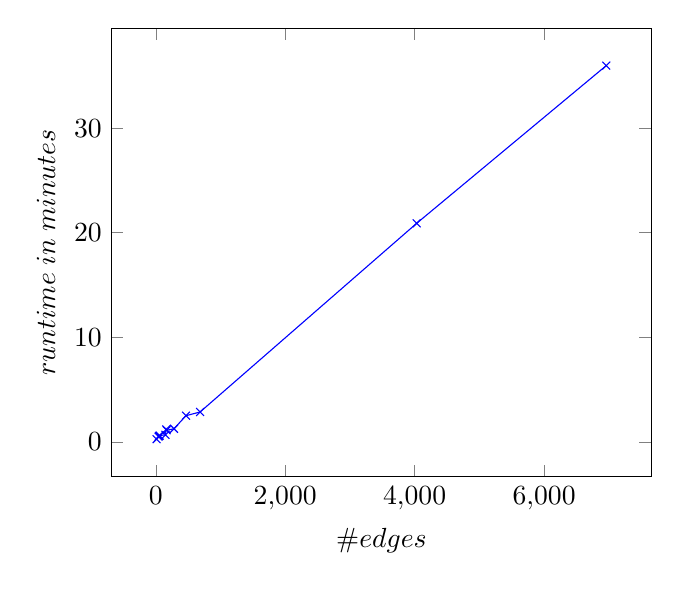
\begin{tikzpicture}
	    \begin{axis}[
	    	xlabel=$\# edges$,
	    	ylabel=$runtime\;in\;minutes$]
	    \addplot[color=blue,mark=x] coordinates {
	    	(12,0.25)
	    	(42,0.5)
	    	(53,0.55)
	    	(61,0.6)
	    	(150,0.67)
	    	(161,1.19)
	    	(167,1.1)
	    	(281,1.25)
	    	(467,2.5)
	    	(684,2.85)
	    	(4031,20.9)
	    	(6961,35.99)
	    };
	    \end{axis}
	  \end{tikzpicture} 
	  \label{rtm}
	  \caption{Runtime in minutes for different amounts of edges, all with 2 million displacement steps}
	\end{figure}
In Figure~\ref{rtm} the runtime of $2$ million displacement steps broken down to the individual graphs can be found. Somewhat expectedly the runtime is linear on the number of edges. Going back to the actual results provided in Table~\ref{best-res} it becomes clear that most time is spend the last two graphs. While a stopping criterion may improve the runtime for the first few minutes, these large graphs likely will not achieve their minimal crossing number within the given time frame. Adding any other operation on top of the displacement step would provide no benefit for these graphs and the seconds saved in the beginning would be counterweighted by the minutes lost later on. Given an environment without a time limit a stopping criterion would improve the algorithm as no specific iteration number would be needed.


    \section{Conclusion}
	In this work a simple algorithm mostly based on randomness is presented. While its performance seems promising, there are still many things to be experimented with which would simply not fit into the scope of this project. The major take-away should be that random algorithms can be both easy to understand and yield competitive results. Throughout the development it proved time and time again that to much restrictions only seem to worsen the result and the simplest approach is the best one: Leaving the randomness as much room as possible by only directing it in such a way that nothing outside of the confinements of the task can be produced. A final word on the contest itself cannot be given at this time as the contest is still to be held.
	Future algorithms building upon this work should keep in mind that many decisions made are purely based on the restrictions of the contest and should be changed accordingly as necessary. The choice of base drawing algorithm is especially important to rethink based on new requirements. As overthinking the algorithm itself would most likely not improve the results by much it is suggested that more time is spend with the actual implementation and its efficiency as well as the approach to parallelization. Nothing improved the results as much as drastically increasing the number of random displacements or simply testing multiple different random seeds in the given time frame.

    \printbibliography
\end{document}
